% HamClock-Next Quick Start Guide
% Build: cd docs/quickstart && pdflatex HamClock-Next-QuickStart.tex
%        cp HamClock-Next-QuickStart.pdf ../
\documentclass[twocolumn,9pt,letterpaper]{article}

\usepackage[margin=0.45in,top=0.35in,bottom=0.35in]{geometry}
\usepackage{graphicx}
\usepackage[table,dvipsnames]{xcolor}
\usepackage{tabularx}
\usepackage{booktabs}
\usepackage[utf8]{inputenc}
\usepackage[T1]{fontenc}
\usepackage{helvet}
\renewcommand{\familydefault}{\sfdefault}
\usepackage[framemethod=TikZ]{mdframed}
\usepackage{enumitem}
\usepackage{microtype}
\usepackage{array}
\usepackage{setspace}
\usepackage{pifont}
\newcommand{\circone}{\ding{172}}
\newcommand{\circtwo}{\ding{173}}
\newcommand{\circthree}{\ding{174}}
\newcommand{\circfour}{\ding{175}}
\newcommand{\circfive}{\ding{176}}

% ── Colours ──────────────────────────────────────────────────────────────────
\definecolor{hcamber}{HTML}{F5A623}
\definecolor{hcdark}{HTML}{111111}
\definecolor{hclight}{HTML}{F0F0F0}
\definecolor{migbg}{HTML}{1E2030}

% ── Section header command ────────────────────────────────────────────────────
\newcommand{\hcsection}[1]{%
  \vspace{4pt}%
  \noindent\colorbox{hcamber}{\parbox[t]{\dimexpr\columnwidth-2\fboxsep\relax}{%
    \color{white}\bfseries\small\strut\enspace #1\strut}}%
  \vspace{3pt}\par\noindent
}

% ── Layout tweaks ─────────────────────────────────────────────────────────────
\setlength{\columnsep}{0.18in}
\setlength{\parindent}{0pt}
\setlength{\parskip}{1.5pt}
\setlength{\extrarowheight}{1pt}
\setlength{\tabcolsep}{3pt}
\pagestyle{empty}

% ── Image path ───────────────────────────────────────────────────────────────
\graphicspath{{../wiki/images/}}

% ── Framed box styles ─────────────────────────────────────────────────────────
\mdfdefinestyle{migbox}{
  backgroundcolor=migbg,
  linecolor=hcamber,
  linewidth=1.2pt,
  roundcorner=3pt,
  innerleftmargin=5pt,
  innerrightmargin=5pt,
  innertopmargin=4pt,
  innerbottommargin=4pt,
  skipabove=4pt,
  skipbelow=0pt
}
\mdfdefinestyle{keybox}{
  backgroundcolor=hclight,
  linecolor=hcamber,
  linewidth=0.8pt,
  roundcorner=3pt,
  innerleftmargin=5pt,
  innerrightmargin=5pt,
  innertopmargin=4pt,
  innerbottommargin=4pt,
  skipabove=4pt,
  skipbelow=0pt
}

\begin{document}

% ═══════════════════════════════════════════════════════════════════════════════
%  PAGE 1 — full-width header: title bar + annotated layout screenshot
% ═══════════════════════════════════════════════════════════════════════════════
\twocolumn[{%
  \noindent\colorbox{hcdark}{\parbox{\linewidth}{%
    \vspace{3pt}\centering
    {\color{hcamber}\LARGE\bfseries HamClock-Next}\quad
    {\color{white}\large Quick Start Guide}\\[1pt]
    {\color{hclight}\footnotesize
      Real-time amateur radio dashboard\,---\,HF propagation, DX spots,
      space weather \& satellite tracking%
    }
    \vspace{3pt}
  }}%
  \vspace{4pt}

  \noindent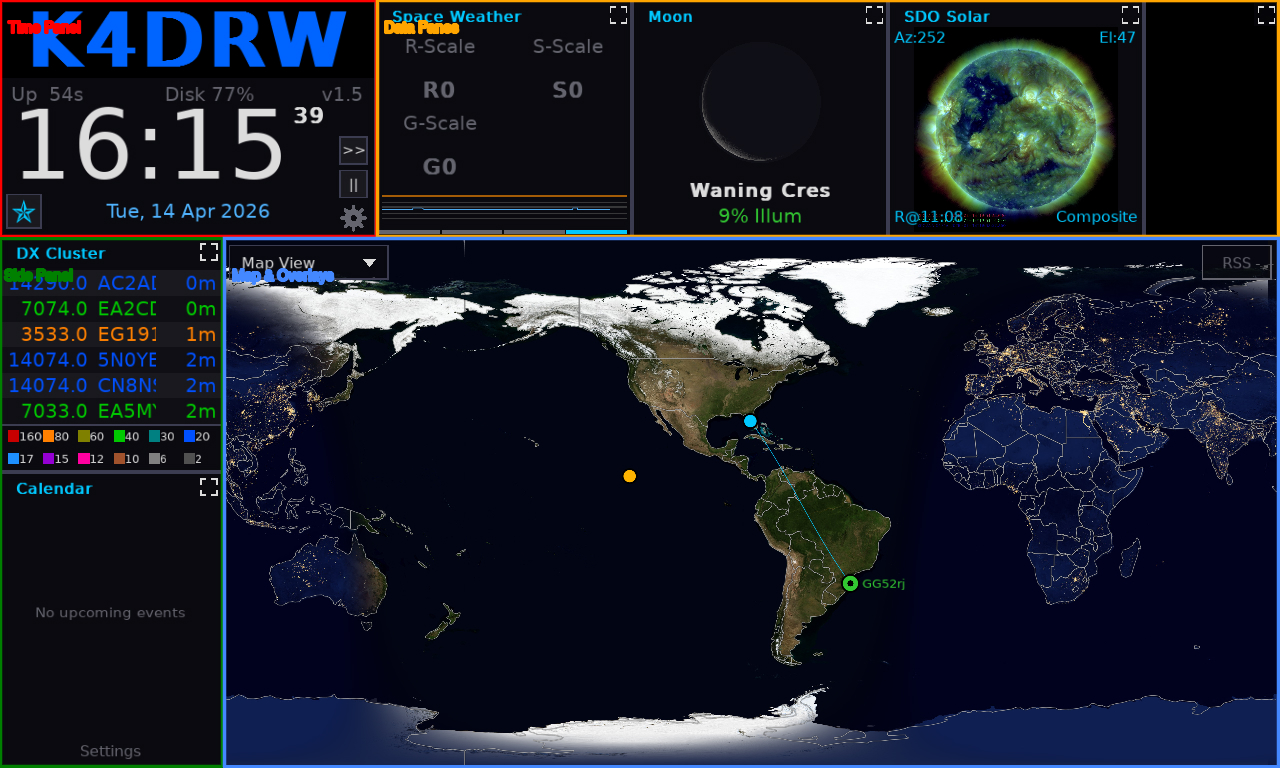
\includegraphics[width=\linewidth,keepaspectratio]{layout-annotated.png}

  \noindent{\footnotesize\color{hcdark}
    \textbf{\circone\,Time Panel} (callsign, UTC/local time, gear\,settings icon)\enspace
    \textbf{\circtwo\,Top Panes} x4 (click coloured strip to pick widget)\enspace
    \textbf{\circthree\,Side Panes} x2\enspace
    \textbf{\circfour\,Map}\enspace
    \textbf{\circfive\,RSS Ticker}%
  }
  \vspace{6pt}
}]

% ─── COLUMN 1 — Settings Menu ────────────────────────────────────────────────
\hcsection{Settings Menu}

Open: click the \textbf{gear} icon in the Time Panel (top-right).

Press \raisebox{0pt}{\colorbox{hcamber}{\color{hcdark}\footnotesize\bfseries\,K\,}} to
enter \textbf{Highlight Mode} --- cyan outlines every clickable element with a tooltip.

\vspace{2pt}
{\footnotesize
\begin{tabularx}{\columnwidth}{@{}>{\bfseries}lX@{}}
\toprule
Tab & Configure \\
\midrule
Identity   & Callsign, grid square, lat/lon, GPS, timezone \\
Appearance & Theme, map style, projection, brightness, units \\
Spotting   & DX cluster host/port, WSJT-X feed, PSK Reporter, RBN \\
Rig/Rot    & rigctld \& rotctld host:port, auto-tune, auto-track \\
Services   & QRZ credentials, RepeaterBook API key, Winlink call \\
Network    & Hub mode (off/server/client), hub IP:port \\
Widgets    & Assign widgets to panes, rotation interval, sync \\
Watchlist  & Callsign watch list, POTA/SOTA activity filters \\
Update     & Check for and download app updates \\
\bottomrule
\end{tabularx}
}

\vspace{3pt}
\noindent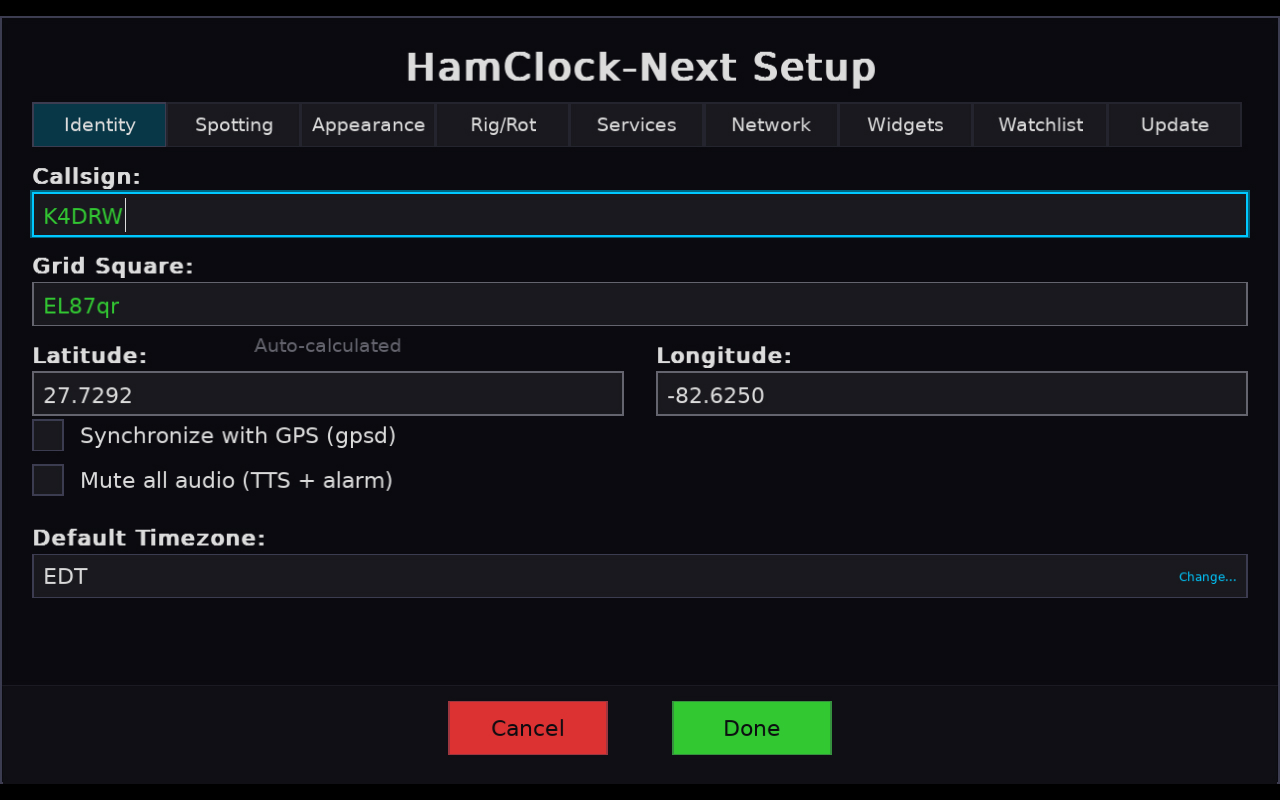
\includegraphics[width=\columnwidth]{modal-setup.png}

% ─── COLUMN 2 — Map View Menu ────────────────────────────────────────────────
\hcsection{Map View Menu}

Open: click the \textbf{Map View} button in the upper-left corner of the map.

\vspace{2pt}
{\footnotesize
\begin{tabularx}{\columnwidth}{@{}>{\bfseries}lX@{}}
Projections   & Equirectangular · Robinson · Azimuthal · Mercator · Dual~Az \\
Map Style     & NASA Blue Marble · Topo · Topo\,+\,Bathy \\
Grid          & Off · Lat/Lon · Maidenhead \\
Prop Overlay  & None · MUF-RT · VOACAP · Reliability · Heatmap · DRAP · Aurora \\
Weather       & None · WX/Pressure · Clouds (GFS) \\
VOACAP params & Band, Mode, Power, TOA, Antenna Gain, Short/Long path \\
Toggles       & Beacons · Borders · Center Map on DE \\
Map Interact  & Scroll wheel\,=\,zoom\enspace Click-drag\,=\,pan\enspace Right-click\,=\,set DE \\
\end{tabularx}
}

% ═══════════════════════════════════════════════════════════════════════════════
%  PAGE 2 — onecolumn: full-width header + side-by-side minipages
% ═══════════════════════════════════════════════════════════════════════════════
\clearpage
\onecolumn

% Full-width amber Widgets banner
\noindent\colorbox{hcamber}{\parbox{\linewidth}{%
  \vspace{2pt}\centering{\color{white}\large\bfseries Widgets}\vspace{2pt}
}}

\vspace{3pt}
{\small
  Click the \textbf{coloured strip} at the top of any pane to open the Widget Selector.
  Each pane holds a \textbf{rotation list} --- add multiple widgets and they cycle
  automatically. Set the rotation interval in \textbf{Settings\,\textgreater\,Widgets}.
  To \textbf{configure a widget}, click the \textbf{lower portion} of the widget
  (e.g., click where it says \textit{Counts} in Live Spots to open its setup).
}
\vspace{4pt}

\noindent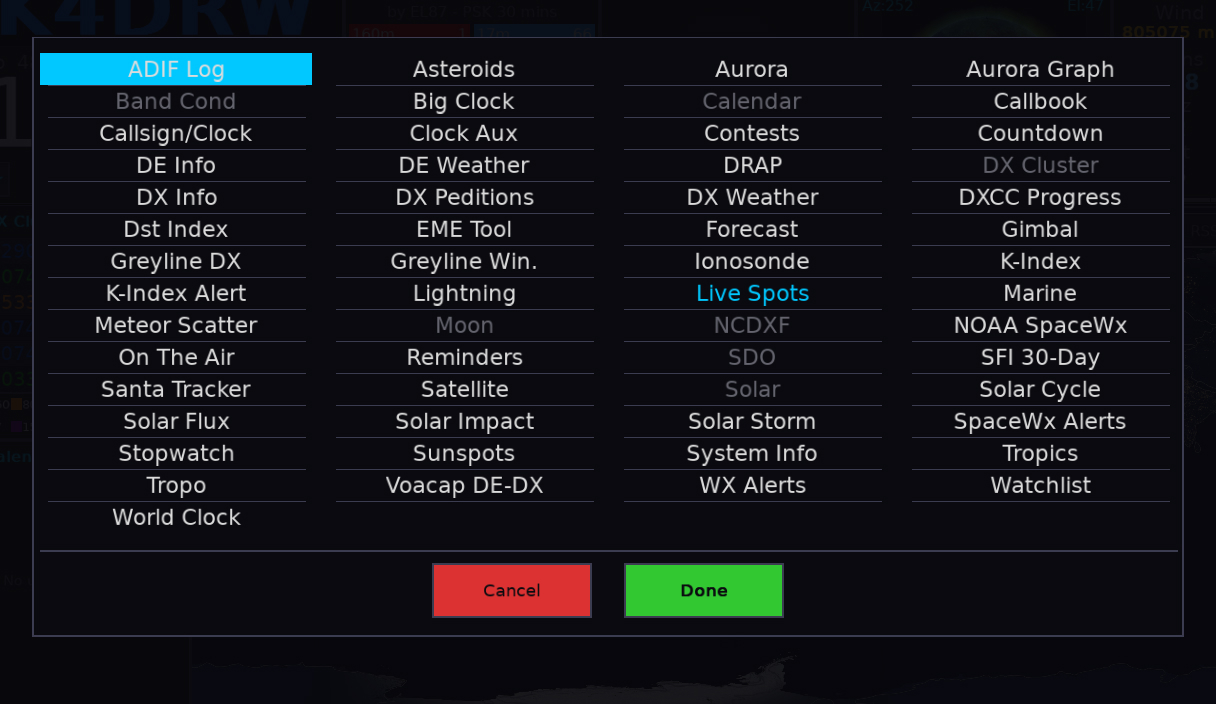
\includegraphics[width=\linewidth,keepaspectratio]{modal-widget-selector.png}

\vspace{6pt}

% ── Side-by-side minipages ────────────────────────────────────────────────────
\noindent
\begin{minipage}[t]{0.495\linewidth}

  % Redefine \hcsection width for minipage context
  \def\mpcw{\linewidth}

  \noindent\colorbox{hcamber}{\parbox[t]{\dimexpr\linewidth-2\fboxsep\relax}{%
    \color{white}\bfseries\small\strut\enspace Widget Categories\strut}}
  \vspace{3pt}\par\noindent

  {\footnotesize
  \begin{tabularx}{\linewidth}{@{}>{\bfseries\color{hcamber}}lX@{}}
  Space Weather  & Solar flux, SDO imagery, Aurora, DRAP, Solar Storm, K-Index \\[5pt]
  Propagation    & Band Conditions, Live Spots, VOACAP DE-DX, Tropo, Meteor \\[5pt]
  DX / Spots     & DX Cluster, Greyline DX, DXpeditions, On The Air (POTA/SOTA) \\[5pt]
  Tracking       & Satellite, Moon, EME Tool, Gimbal (rotator), Asteroid \\[5pt]
  Weather        & DE/DX Weather, Lightning, Hurricane, Marine (tides/AIS) \\[5pt]
  Clocks \& Info & Big Clock, World Clock, Calendar, DE/DX Info, Callbook \\[5pt]
  Timers         & Countdown, Stopwatch, Reminders \\[5pt]
  Contests       & Contest Schedule, Propagation Forecast \\[5pt]
  Environment    & Temp, Pressure, Humidity, Dew Point (BME280 I\textsuperscript{2}C) \\
  \end{tabularx}
  }

  \vspace{5pt}
  \noindent\colorbox{hcamber}{\parbox[t]{\dimexpr\linewidth-2\fboxsep\relax}{%
    \color{white}\bfseries\small\strut\enspace Coming from the original HamClock?\strut}}
  \vspace{3pt}\par\noindent

  \begin{mdframed}[style=migbox]
    {\color{hclight}\footnotesize
    \begin{itemize}[leftmargin=1em,itemsep=2pt,topsep=0pt,parsep=0pt]
      \item \textbf{Panes replace fixed slots} --- each pane rotates a configurable widget list
      \item \textbf{Settings are GUI-based} --- no direct JSON file editing required
      \item \textbf{Map overlays \& projections} live in the right-click Map View Menu
      \item \textbf{PSK Reporter} ``of DE'' mode preserves original HamClock behaviour
      \item \textbf{All original data sources} are present; callsign/grid carry over
    \end{itemize}
    }
  \end{mdframed}

\end{minipage}
\hfill
\begin{minipage}[t]{0.485\linewidth}

  \noindent\colorbox{hcamber}{\parbox[t]{\dimexpr\linewidth-2\fboxsep\relax}{%
    \color{white}\bfseries\small\strut\enspace Quick Keys\strut}}
  \vspace{3pt}\par\noindent

  \begin{mdframed}[style=keybox]
    {\small
    \begin{tabularx}{\dimexpr\linewidth-2\fboxsep-2\fboxrule\relax}{@{}>{\bfseries\ttfamily}lX@{}}
    K        & Highlight Mode --- cyan outlines all clickable elements \\[5pt]
    ?        & In-app help overlay \\[5pt]
    F11      & Toggle fullscreen \\[5pt]
    Ctrl+Q   & Quit application \\[5pt]
    Arrows   & Scroll satellite list (when satellite pane active) \\[5pt]
    PgUp/Dn  & Page through satellite list \\
    \end{tabularx}
    }
  \end{mdframed}

  \vspace{6pt}
  \noindent\colorbox{hcamber}{\parbox[t]{\dimexpr\linewidth-2\fboxsep\relax}{%
    \color{white}\bfseries\small\strut\enspace Get Help\strut}}
  \vspace{3pt}\par\noindent

  \begin{mdframed}[style=keybox]
    {\small
    \begin{tabularx}{\dimexpr\linewidth-2\fboxsep-2\fboxrule\relax}{@{}lX@{}}
    \textbf{Full Wiki}    & \texttt{github.com/k4drw/hamclock-next/wiki} \\[4pt]
    \textbf{Widget Setup} & Settings\,\textgreater\,Widgets tab in-app \\[4pt]
    \textbf{Tip}          & Press \textbf{K} then hover any element for a one-line description \\
    \end{tabularx}
    }
  \end{mdframed}

\end{minipage}

\vfill
\noindent\colorbox{hcdark}{\parbox{\linewidth}{%
  \vspace{4pt}\centering
  {\color{hcamber}\small\bfseries HamClock-Next v1.5}\enspace
  {\color{hclight}\small\texttt{github.com/k4drw/hamclock-next}}\enspace
  {\color{gray}\small Released 2026}%
  \vspace{4pt}
}}

\end{document}
